\chapter{Theory}
\label{chap:theory}

% -------------------------------------------------------------------------------------------------
%                                            Structure
% -------------------------------------------------------------------------------------------------

% - Reiteration of Idea       -> Was wird hier gemacht    -> Was benötigt man dafür

% - Impl Platform             -> Was provided die Hardware und Plattform schon, Was braucht es noch?

% - Implementation Steps      -> Overview over the implementation chapter (but without the single address cases)

% -Übersicht über die benötigten Änderungen
%     - TLB Miss Exception
%         - Exceptions and TLBS in RISC-V
%         - New Exception
%         - Vorlage: MIPS
%             - Riscv Exception basics (if not in fundamentals)
%             - New Exceptions? -> Was man beachten muss


%      - Exception Handler in general
%             - General Stuff, xv6 Exception Handler
%             - Vectored
%             - All registers that come into play
%             - xv6 book, exception machinery

%         - Exception Handler for the TLB Miss exception

%     - TLB Filling
%         - Vorlage MIPS

%         - RISCV CSRs -> Extensibility


%         - QEMU TLB


%         - Concrete CSRs for TLB filling (THIS IS THE RESULT OF THIS CHAPTER)
%             (- TLB Flushing, Replacement policy (vs mips))


%     - Mapping functions
%         - Segmented
%         - More?


% -------------------------------------------------------------------------------------------------
%                                            Intro
% -------------------------------------------------------------------------------------------------
% Überblick über die Idee schaffen -> Virtueller Speicher durch funktion möglich


This chapter presents the theoretical foundation of the the implementation presented in the next chapter.
It will start with a short elaboration on the general idea followed by a description of the
programming platform.
It then presents the theory behind the different components of the implementation.
% Then?

% -------------------------------------------------------------------------------------------------
%                                            Idea
% -------------------------------------------------------------------------------------------------
% Beantwortet die Frage: Was wird hier überhaupt gemacht? (Ohne zu sehr ins detail zu gehen)
% Auch die Motivation und was das Ergebnis sein könnte/ erwartet ist



\section{Function-based Virtual Memory}
% Idea Description

% The implementation is not only about the mapping functiion but also about the  platform modifications to create mapping functions

The goal of this work is to provide a proof of concept of an alternative approach
to Virtual Memory management that reduces the overhead associated with traditional page tables walks.
Instead of suffering the penalty of up to five memory accesses on a TLB miss,
we want to explore using simple functions for the mapping.

Figure \ref{fig:theory:normal_tlb_miss} shows the usual architecture of a system
with a hierarchical page table.
This architecture provides only limited flexibility in interacting with the TLB, especially when it comes to TLB writes.
Architectures like MIPS allow direct manipulation of TLB structures and thus provide a good framework for implementing new approaches for Virtual Memory management.

The architecture is only one half of the design. To test the ideas for mapping
functions, a system utilizing the memory system and defining the functions is necessary.
The xv6 educational operating system provides a good platform for experimentation as it is very lightweight and provides a Unix-like interface and structures.

xv6 is designed for RISC-V, but RISC-V does not allow for flexible software-management of the TLB structure.
Thus part of this chapter will describe the theoretical foundations for modifying
the QEMU/RISC-V emulator to transform the memory system architecture to something
more similar to MIPS.
The final architecture for the memory system will look like depicted in figure \ref{fig:theory:mapping_fx}
% TODO der Zwischenschritt mit dem Software Page Table walk wird dann in der Impl
% eingeführt

% Normal Page Table Walk
\begin{figure*}[ht!]
    \centering
    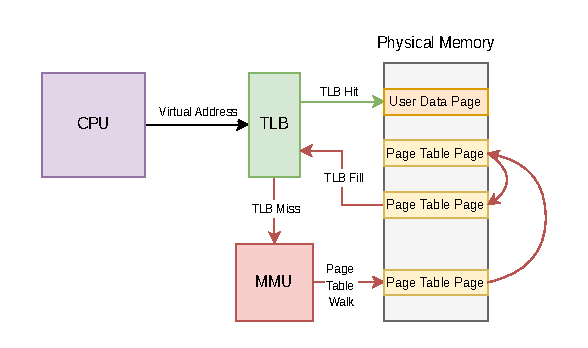
\includegraphics[scale=1.5]{figures/theory_normal_tlb_miss.pdf}
    \caption[Usual TLB Miss]{This figure shows what usually happens when the TLB misses:
        the miss will invoke the hardware state machine page table tree walker; the walker traverses
        the page table tree and if a valid PTE is found, the mapping is added to the TLB. The processor
        then executes the failing instruction again which will then result in a TLB hit}
    \label{fig:theory:normal_tlb_miss}
\end{figure*}
% Virtual Memory using a Mapping Function
\begin{figure*}[t]
    \centering
    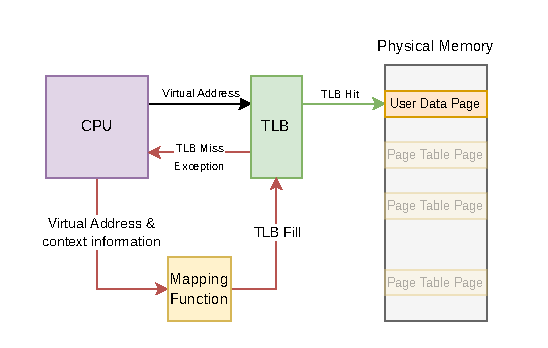
\includegraphics[scale=1.5]{figures/theory_mapping_fx.pdf}
    \caption[Virtual Memory using a mapping function]{Instead of emulating a hardware page table walk in software on
        a TLB Miss exception, a mapping function is invoked that calculates the PTE using arithmetic primitives and tries
        to avoid memory references.}
    \label{fig:theory:mapping_fx}
\end{figure*}

To adapt the RISC-V emulator to fit the architectural design, a number of changes to the implementation of the emulator are necessary:

\begin{itemize}
    \item Extending the Qemu emulator to trigger an exception on a TLB miss
    \item A machine-mode trap handler in xv6 that handles the TLB miss exception
    \item A way to write TLB entries using special instructions
\end{itemize}


% -------------------------------------------------------------------------------------------------
%                                            Platform
% -------------------------------------------------------------------------------------------------
% Answers: Welche Platform wird verwendet? Warum?  Was provided die Platform, was nicht?
\section{Platform}
The chosen platform is the xv6 operating system \cite{xv6source}. It is a teaching operating system
used by MIT operating systems courses to teach the basics of operating systems.
xv6 implements the basic Unix Version 6 interfaces, but does so in a very simplified fashion.
There is an x86 version and a RISC-V version. For this project, the RISC-V version was chosen.
xv6's simplicity and the accompanying handbook \cite{cox2011xv6} make it a good choice for a first
proof of concept.

xv6 will be run on the QEMU \cite{QEMUSource2024} emulator. The QEMU RISC-V emulator implements
all the RISC-V features and extensions that xv6 needs.

Since using actual RISC-V hardware is not possible within the scope of implementing a new exception, an emulator is used to implement and utilize the necessary changes to the ISA. The QEMU emulator was chosen for this purpose, as it is very comprehensive and performant, and also emulates a TLB.


% Was provided die Platform noch nicht, was muss noch gemacht werden um das Design zu realisieren?
% Implications of programming platform on implementation -> needing to implement TLB Miss
% -------------------------------------------------------------------------------------------------
% -------------------------------------------------------------------------------------------------
%                                            IMPL THEORY
% -------------------------------------------------------------------------------------------------
% -------------------------------------------------------------------------------------------------


% -------------------------------------------------------------------------------------------------
%                                            TLB MISS EXCEPTION
% -------------------------------------------------------------------------------------------------
% -------------------------------------------------------------------------------------------------
\section{TLB Miss Exception}
Operating systems running on RISC-V hardware are not directly notified of TLB misses.
A TLB miss can only be inferred when a page fault occurs. Otherwise, TLB misses will be handled
by the MMU.
To manage a TLB in software the operating system needs to be made aware that a TLB miss occured.
The natural mechanism to do this is the exception mechanism.

% -------------------------------------------------------------------------------------------------
\paragraph{RISC-V Exceptions}
Unlike MIPS \cite{heiserAnatomyHighPerformanceMicrokernel}, RISC-V does not raise a TLB miss exception on TLB miss.
Instead, the \emph{Virtual Address Translation Process} is initiated: The MMU will walk through
the page table tree and may, depending on the PTEs, either throw different kinds of page faults, or
successfully add the missing entry to the TLB.
At this point the faulting instruction will either be repeated, if the TLB fill was successful, or
a page fault exception will be invoked \cite{RISCVInstructionSet}. The kernel then has to handle that page fault with help
of the contents of the \texttt{satp} and \texttt{mtval} (or \texttt{stval}) registers.

The behavior of a TLB Miss exception should be pretty similar: If the TLB hits, the program will
just continue as usual. If the TLB misses, an exception should be raised, providing context
information about the miss in registers. The invocation of the hardware page table walker is
not necessary.


% -------------------------------------------------------------------------------------------------
\paragraph{Adding a new Exception to RISC-V}
Extending the emulator to throw a new exception is explained in the Implementation chapter.
On the theoretical side, it is important to choose an exception code from the code ranges designated
for custom use. These are $24-31$ and $48-63$ \cite{RISCVInstructionSet}. For the implementation we chose $24$ or $0x18$.



% -------------------------------------------------------------------------------------------------
%                                            Exception Handling
% -------------------------------------------------------------------------------------------------

% -------------------------------------------------------------------------------------------------
\section{Exception Handling}
Throwing an exception is only part of the design. The operating system also has to handle the exception appropriately.

% -------------------------------------------------------------------------------------------------
\paragraph{L4/MIPS TLB Exception Handling}
MIPS vectors its exception vectors in a continuous area in memory, starting at a base address.
That gives the TLB miss handler 32 instructions to service the TLB Miss. Otherwise it has to jump
somewhere with more space.
The \emph{Fast TLB Miss} handler is able to service the miss using only the two kernel-reserved
registers \texttt{k0} and \texttt{k1} and another register, which has to be saved first \cite{heiserAnatomyHighPerformanceMicrokernel}.
Thus the memory footprint of the handler is low.

% -------------------------------------------------------------------------------------------------
\paragraph{xv6 Exception Handler}
xv6's exception handler does not actually handle most exceptions. For most exceptions,
but notably also the different page fault exceptions, xv6 will simply kill the offending process \cite{cox2011xv6}.

% -------------------------------------------------------------------------------------------------
\paragraph{TLB Miss Exception Handler}
To simplify things, we will let the TLB Miss exception handler run in machine mode only.
The usual mode for a operating system kernel would be the supervisor mode. However, this
mode also uses address translation. This could create a situation in which we would have
to deal with nested exceptions.

\paragraph{Catching the Exception} M-mode exceptions will set the program counter to the address
specified in the \texttt{mtvec} register. Originally, xv6 only serviced the asynchronous
timer interrupt in machine mode. Every other trap is forwarded to supervisor mode.
The trap vectoring mode can also be changed by setting the \texttt{MODE} field of the
\texttt{mtvec} register \cite{RISCVInstructionSet}. The alternative mode forwards
each interrupt to its own address, set at a fixed offset from the \texttt{BASE} address.
\todo{mtvec bytefield}

Every exception will still be forwarded to the \texttt{BASE} address set in the \texttt{mtvec}
register, regardless of the vectoring mode.

The value of the \texttt{mcause} register identifies the reason for the exception.
This value can be used in something like a switch-case statement to call specific handlers
for the different exception causes.
This switch-case is not necessary in xv6, since the only exception that can enter
the machine-mode exception handler is the TLB Miss exception.

Before running any code that modifies general-purpose registers, the current state of the
registers and the program counter should be saved to memory. These need to be restored after
the exception handler code has finished.
This is essential to keep the process, that was just running when the exception triggered,
in an consistent state when execution resumes.


% -------------------------------------------------------------------------------------------------
%                                            TLB FILLING
% -------------------------------------------------------------------------------------------------
\section{TLB Filling}
Not only does the operating system need to be made aware of TLB misses,
the operating system also needs to be able to write to the TLB to actually create
mappings that will be used after the handler finishes.
RISC-V also does not provide any means to write to the TLB out of the box. But the RISC-V Control and Status Registers
(CSRs) allow for a great deal of extensibility \cite{riscvreader}.
With CSRs, it is possible to implement custom behavior, which can then be accessed using instructions
of the \texttt{CSRR} instruction group.
To make an informed decision on how the CSR format for TLB writing may look like, we will first
look at the TLB and the TLB instructions of \emph{MIPS}. Then we will take a look at what the
RISC-V ISA specifies about TLB, how QEMU implements TLBs and finally we will look at the
CSR format that is used for the implementation.

% -------------------------------------------------------------------------------------------------
\subsection{MIPS TLBs}               % Combine TLB Sections into one ( Multiple TLB designs clash here ...)

%       Starting with MIPS for inspiration on how instructions for TLB manipulation may look like
%       Then continue with a possible RISCV Implementation Idea
%       I-TLB and D-TLB out of scope
% Inspiration: MIPS

The MIPS64 instruction set manual \cite{MIPSArchitectureProgrammers2016}
shows a number of different instructions concerned with invalidation, probing, flushing, reading
and writing (indexed and random) of the TLB.
The most interesting instruction for a first design would be the \texttt{TLBWR} instruction for writing a TLB
entry at a random index. With a similar instruction in RISC-V, we can already implement a purely
software-controlled VM system.
The other types of TLB instructions that MIPS provides are not strictly necessary,
except for flushing. Without being able to flush existing translations from the TLB,
user mode processes may try to access physical mappings stemming from other processes. But the RISC-V privileged architecture already provides this functionality
with the \texttt{sfence.vma} instruction \cite{riscvreader}.


% Replacement policy
%   MIPS -> Indexed writes
\paragraph{Replacement Strategies} An advantage of software-managed TLBs is that the operating system can implement custom
TLB replacement policies, that may even change depending on workload, programs running
and other circumstances.
The default replacement strategy for the MIPS \texttt{tlbwr} instruction is to simply
use the value of the \texttt{C0\_RANDOM} register as the index for the next TLB entry
to be replaced. The name of that register is misleading, because it is not actually a
random value, but it is rather decremented on each instruction \cite{heiserAnatomyHighPerformanceMicrokernel}.
It is not clear whether this is a sensible replacement strategy,
but it can be used to ensure that the same TLB slot is not used for every \texttt{tlbwr} if the implementation
does not provide for any further replacement strategy.
Some TLB entries can be protected from this ``random'' replacement by setting a value in the \texttt{C0\_WIRED}
register. The value in this register represents a lower bound, protecting all TLB entries that lie below it.
This is useful to keep some mappings in the TLB that are valid all the time.

% TODO should this be here? We should probably have a discussion about xv6 first
%Protected TLB entries in xv6 -> Trampoline page
Having a protected space of TLB entries can especially be useful for global mappings. xv6 employs such a global
mapping for every process and the kernel with the trampoline page.\todo{trampoline page should be explained in fundamentals/platform}

\paragraph{MIPS - TLBWR} The arguments for the instruction need to be written in some
other registers - \texttt{EntryHi}, \texttt{EntryLo0}, \texttt{EntryLo1} and \texttt{PageMask}.
The contents of those registers directly correspond to the TLB entry, which creates quite large
TLB entries \cite{heiserAnatomyHighPerformanceMicrokernel}.



% -------------------------------------------------------------------------------------------------
\subsection{TLB CSRs}
The minimum information the hardware needs to create a mapping is the faulting physical address and
the virtual address it maps to.
The mapping has a granularity of 4 KB pages. Thus, the lower 12 bits of both the physical and the
virtual address are not needed.
This still leaves $2*(64-12)=104$ bits for the mapping.
The virtual address cannot be easily shortened further. Taking some of the most significant bits
would shorten the Virtual Memory space of the programs.
The physical address could still be shortened to only have enough bits to cover the physical address
space used by xv6.
But this would still end up taking more than 64 bit and thus more than one CSR.

So instead of trying to save as much space as possible, two CSRs are used.
This also leaves enough room for more experimentation with the format.
They are called \texttt{tlbwh} (TLB Write High) and \texttt{tlbwl} (TLB Write Low).
The emulator will expect the physical address \ref{fig:theory:sv39pa} in \texttt{tlbwh} and a the virtual address in form
of a PTE \ref{fig:theory:sv39pte} in the \texttt{tlbwl} CSR.
% Fixed TLB format, but flexibilty of CSR format


% TLBH
\begin{figure*}[t]
    \centering
    \begin{bytefield}[bitwidth=\widefigurewidth/64,bitheight=\widthof{~PBMT~}, bitformatting={\tiny\bfseries}, boxformatting={\centering}]{64}
        \bitheader[endianness=big]{63,38,11,0} \\
        \bitbox{25}{Unused}&
        \bitbox{27}{VPN}&
        \bitbox{12}{Page Offset}
    \end{bytefield}
    \caption[TLBH CSR Format]{\textbf{TLBH CSR Format} The format is derived from the format of Sv39 virtual addresses and also works for Sv48 and Sv57 virtual addresses by keeping the most significant bits unused}
    \label{fig:theory:tlbh}
\end{figure*}

%TLBL
\begin{figure*}[h!]
    \centering
    \begin{bytefield}[bitwidth=\widefigurewidth/64,bitheight=\widthof{~PBMT~}, bitformatting={\tiny\bfseries}, boxformatting={\centering}]{64}
        \bitheader[endianness=big]{63,53,9,8,7,6,5,4,3,2,1,0} \\
        \bitbox{10}{Unused} &
        \bitbox{44}{PPN} &
        \bitbox{2}{\rotatebox{90}{RSW}} &
        \bitbox{1}{D} &
        \bitbox{1}{A} &
        \bitbox{1}{G} &
        \bitbox{1}{U} &
        \bitbox{1}{X} &
        \bitbox{1}{W} &
        \bitbox{1}{R} &
        \bitbox{1}{V}
    \end{bytefield}
    \caption[TLBL CSR Format]{\textbf{TLBL CSR Format} The format is derived from the Sv39 PTEs. Reserved bits at the top are omitted. Access rights are retained to be set in the TLB}
    \label{fig:theory:tlbl}
\end{figure*}



% -------------------------------------------------------------------------------------------------
%                                            MAPPING FUNCTION
% -------------------------------------------------------------------------------------------------
\section{Mapping Functions}
% -------------------------------------------------------------------------------------------------
\subsection{Segmented Mapping}

The first attempt at a mapping function based paging design
uses a design that determines memory allocation at compile time.
The resulting mapping is similar to a segmented memory design.

% Elaboration on segmented memory design
\paragraph{Segmeneted Memory}
\textit{Memory Segmentation} splits available memory into logical segments following the structure of a program. Thus there may be a segment for the programs code, the data, stack and so on.
For bookkeeping, there is a segment table keeping track of the base address of the segment
and the size of the segment.
The operating system uses the base address to calculate the physical address from the logical
address consisting of segment number and offset. The segment size is used to ensure that
accesses beyond the segment result in an error \cite{tanenbaumOS}.

The main advantages of this memory design are that the memory layout follows the logical structure of the programs and that the segments are protected from undesired access (like writing to the code segment).
Typical segmented memory designs also allow for dynamic segment sizes \cite{tanenbaumOS}.



% Elaboration on this specific design
\paragraph{Tableless Segmented Virtual Memory}
As a typical segmented memory design splits the programs memory into logical units, this design uses segmentation to split the whole physical memory into logical parts.
These logical parts however do not reflect the structure of a program, but distinct process address spaces: Each segment of main memory can hold one process.
To keep the design as lightweight as possible, each segment has a fixed size, which is determined at compile time of the operating system.
This is less flexible but omits the need of storing the segment size for each segment, as they are all the same size.
To calculate a physical address from a virtual one, all the mapping function needs is the ASID (segment number) and the offset into the address space.
To check whether accesses reach over the the segment, only the static segment size is necessary.

This approach also protects logical units (process address spaces) from each other. This is made sure
by flushing the TLB on context switch.

\todo{figure to visualize this?}

% Segmented memory layout

\begin{figure*}[ht!]
    \centering
    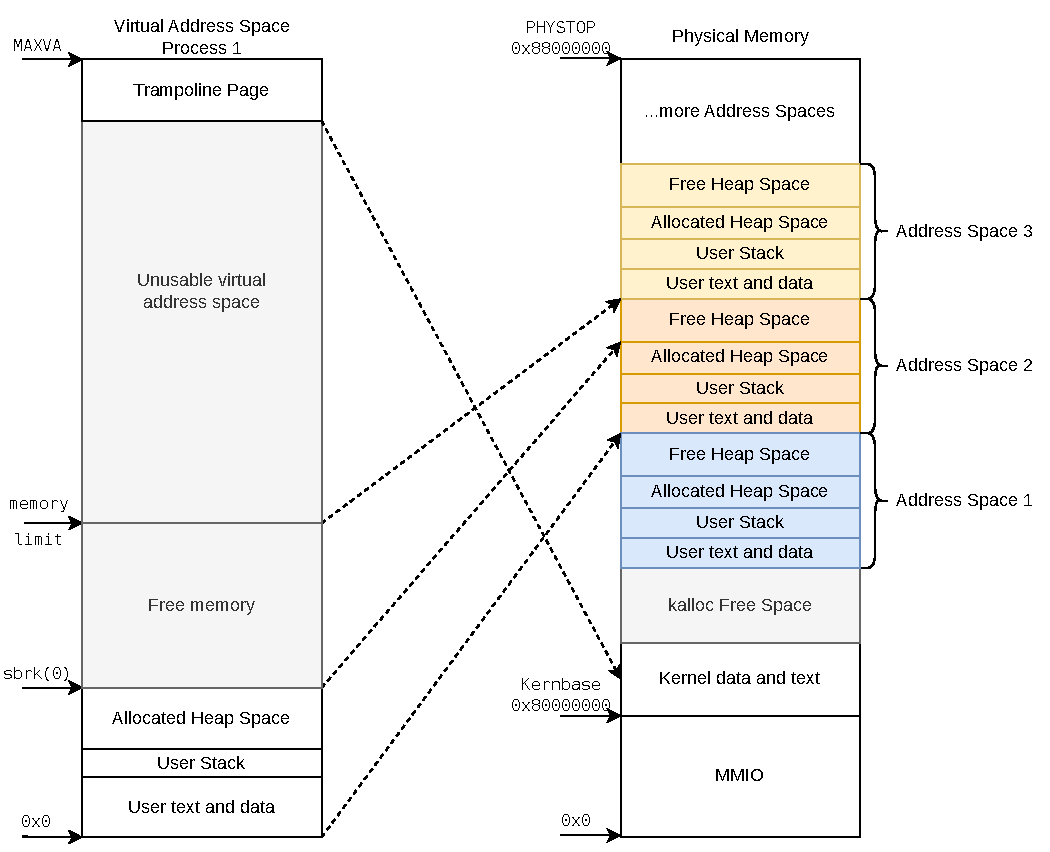
\includegraphics[]{figures/segmented_layout.pdf}
    \caption[Segmented Memory Layout]{\textbf{Segmented Memory Layout}}
    \label{fig:theory:segLayout}
\end{figure*}

% Assumptions
\paragraph{Program Layout} The segmented memory design assumes that programs place their data at the low end of their address
space and grow upwards.
Placement of memory pages at higher addresses than the maximum per-address space memory size does not work. This is a serious restriction to the flexibility of the programmer. Conventional processes load the stack segment at the very top of the virtual address space and the heap segment at the bottom to grant both as much space to grow as possible \cite{tanenbaumOS}. This is still possible with segmentation, but requires context information at compile time about the maximum size of a segment.

xv6 processes do however satisfy these restrictions. Figure \ref{impl:proclayout} shows the memory layout
of an xv6 process.

\begin{marginfigure}
    \centering
    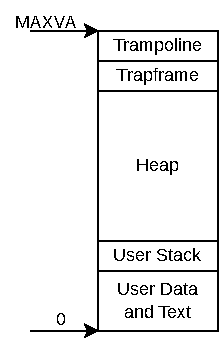
\includegraphics[scale=.8]{figures/prog_vm.pdf}
    \caption[xv6 memory layout]{Virtual memory layout of xv6 processes. Taken from the xv6 book \cite{cox2011xv6}.}
    \label{impl:proclayout}
\end{marginfigure}


\paragraph{Trapframe and Trampoline} xv6 pins special pages to the top end of a processes address space: The trampoline and trapframe pages.
The trampoline page contains code for context switches and kernel entry and needs to be mapped
into every processes address space.
The trapframe is used to save the state of the process on context switch and is thus essential for every process.

In xv6's original memory system, both of these pages would be pinned to the maximum virtual address.
With the segmented design, the address space only comprises the range of \[
    [0 ; MEM\_START+ASID*MAX\_AS\_SIZE]
\]
with \texttt{MEM\_START} being the start of the \texttt{RAM}, \texttt{ASID} being the \emph{Address Space Identifier} of the process and \texttt{MAX\_AS\_SIZE} being the maximum size of one address space.
\texttt{MAX\_AS\_SIZE} is determined by the size of available physical memory divided by the maximum
number of processes that can simultaneously run.

The address space of a process would thus not be big enough to include the usual addresses for the
trapframe and trampoline pages.
To not change the memory layout of xv6 processes, a special rule is put into the mapping function
to explicitly check for the usual addresses of trapframe and trampoline and then map them to appropriate physical addresses.
The trampoline page can be the same for every process, but the trapframe needs to be unique per
process and is thus pinned to the very top of the physical segment of each process.


% Flush not precicse anymore if using more ASs than ASIDs in satp field


% A look at input and output data
% Calculation of addresses

\paragraph{Address Calculation}
The calculation of physical addresses from virtual ones is very straightforward. All that is required is the ASID of the process and the offset into the address space.
The ASID is saved in the process control block (PCB). But because accessing it may be expensive when frequent TLB misses occur, the ASID is encoded into the \texttt{satp} register.
\texttt{satp} is normally used to provide the base address of the root page table to the memory management hardware, but since there is no page table to be used in the memory manager, the register is free to be used for additional context info in the exception handler.

Looking back at figure \ref{fig:theory:sv39satp} shows that there is a ASID field in \texttt{satp} anyways,
so the \texttt{PPN} field does not have to be touched.
But the implementation may choose to use a different number of address spaces than there are supported by the \texttt{ASID} field to allow more processes to be run at the same time.
But with 16 bit, $2^{16} = 65536$ address spaces can be supported, which should be more than enough.

% Assumption: TLB more often than context switch
This optimization is based on the assumption that TLB misses (and thus calls to the exception handler) occur more frequently than context switches, which should be granted when processes use more than one page and have all their TLB entries flushed at context switch.
So the access of the ASID is moved from the frequent TLB miss exception handler to the infrequent context switch. % Heißer 20 year or liedtke homage?

% xv6 Perspective and specifcs (but still theory!) -> Into Impl?
%   Special mappings -> special case in tlb manager (e.g. Trampoline)




% -------------------------------------------------------------------------------------------------
% -------------------------------------------------------------------------------------------------
% -------------------------------------------------------------------------------------------------
% -------------------------------------------------------------------------------------------------
